\documentclass[11pt]{article}

\usepackage[T1]{fontenc}
\usepackage[margin=0.8in]{geometry}
\usepackage{amsmath,amssymb}
\usepackage{graphicx}
\usepackage{wrapfig}
\usepackage{caption}
\usepackage{titlesec}
\usepackage{hyperref}
\graphicspath{{../../../figures/}}

\captionsetup{font=small,labelfont=bf}
\titleformat{\section}{\normalfont\large\bfseries}{}{0pt}{}
\titlespacing*{\section}{0pt}{6pt}{2pt}
\setlength{\parskip}{3pt}
\setlength{\parindent}{0pt}
\pagestyle{empty}

\begin{document}

\begin{center}
{\Large\bfseries Forecasting Sea-Level Rise from Data}\\[3pt]
{\normalsize A summary of Ar\'{e}te's SPECTRUM forecast and its main findings}
\end{center}

\section{Why sea level matters}

Every centimeter of sea-level rise exposes about 1.6 million more people to coastal flooding each year. Planning for future sea levels depends on how well we can forecast them. Most published forecasts come from complex computer models of the ice sheets. These models are not yet able to reproduce observed trends because they represent many physical processes that the available observations cannot calibrate. Their answers therefore depend on assumptions that are currently untestable. As a result, the high-end estimates published in recent years range from 0.6 to 2.0 m of rise by 2100, an untenable range for effective planning.

\section{Our approach}

Sea level rises for a few distinct reasons. Seawater expands as it warms. Mountain glaciers and the Greenland and Antarctic ice sheets lose ice to the ocean. We give each of these contributors its own simple physical model. We test and tune each model with decades of direct observations of that contributor. We call the framework SPECTRUM. The record of global sea level itself is set aside and used only to test the finished forecast. The models never see the answer they are asked to reproduce, which allows the forecast to be validated.

\section{Testing the forecast against the past}

We drove the combined SPECTRUM model with observed temperatures and compared it with observed sea level. Satellites have measured global sea level to millimeter precision since 1993. Over that period, our model matches the observed rate of rise to within 3\%, with an average rate of 3.19 mm of sea-level rise per year. The model also reproduces how the rate of rise has sped up as the planet has warmed since 1940. It captures the shift from a rise driven mainly by warming seawater to one driven mainly by melting ice. That 85-year window spans 1.1 to 1.2 $^\circ$C of warming. The forecast to 2100 covers a similar span of time and a further 1 to 2 $^\circ$C of warming. This demonstration of skill against the past gives us confidence in the forecast of every contributor except one.

The exception is the West Antarctic Ice Sheet, which contributed little in the 20th century but is now home to the fastest-changing glaciers on the planet, including Thwaites Glacier. These glaciers rest on bedrock below sea level, which means once they begin to retreat, their retreat may sustain itself and speed up no matter how quickly we cut emissions. The observed record is too short to tell for sure whether that has begun. We therefore represent West Antarctica with two scenarios. In the first, ice loss continues along its observed path. In the second, ice loss accelerates. The forecast blends the two, and ongoing work is focused on narrowing the forecast for West Antarctic ice loss.

\section{The forecast}

\begin{figure}[t!]
\centering
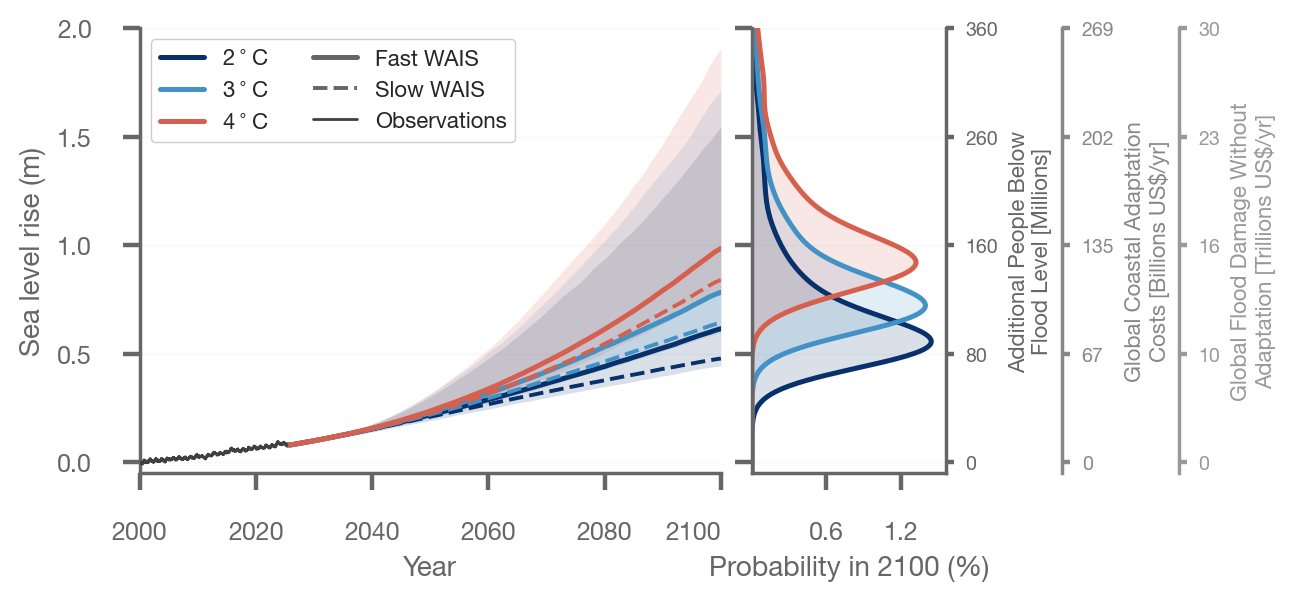
\includegraphics[width=\textwidth]{fig2v4_wais_fan_pdf.png}
\caption{Global sea-level forecast relative to the year 2000 for warming of 2, 3, and 4 $^\circ$C by 2100. The left panel shows the forecast through 2100. Solid lines and shading show the typical outcome and 90\% range of the forecast that includes fast West Antarctic ice loss. Dashed lines show the typical outcome if West Antarctic loss stays slow. The dark gray line shows satellite observations. The right panel shows the chance of each level of rise in 2100 for the forecast that includes fast loss. The right-hand scales convert rise into additional people living below flood level, annual adaptation costs, and annual flood damages without adaptation.}
\label{fig:forecast}
\end{figure}

We drive the SPECTRUM models with three warming trajectories that end near 2, 3, and 4 $^\circ$C above pre-industrial temperatures by 2100. Current policies put us on a path to about 3 $^\circ$C. The typical model outcomes are 0.6, 0.8, and 1 m of rise by 2100 relative to the year 2000 (Fig.~\ref{fig:forecast}). These values are 38 to 44\% higher than the projections of the Intergovernmental Panel on Climate Change, which are known to be biased low. The chance that sea level rises more than 1 m above its pre-industrial level by 2100 is 25\% under 2 $^\circ$C, 44\% under 3 $^\circ$C, and 90\% under 4 $^\circ$C.

\section{Two independent kinds of risk}

The forecast uncertainty has two parts, and each calls for a different response. The first comes from warming seawater, Greenland, and mountain glaciers. These respond to temperature in ways that past observations constrain well, and cutting emissions reduces their contribution. Together they account for about 1\% of the variance in the forecast, virtually all of it from the uncertainty in future emissions. If West Antarctica loses ice slowly, these contributors govern the forecast, and cutting warming from 4 to 2 $^\circ$C would avoid 36 cm of rise. That would spare 61 million people from coastal flood risk and save US\$49 billion per year in adaptation costs.

West Antarctica accounts for 99\% of the forecast variance. That is what we need to worry about because it sets the upper tail, the worst-case scenarios. Cutting warming from 4 to 2 $^\circ$C lowers the typical outcome by 0.37 m but does not retire the risk of more than 2 m of rise. It only lowers that risk from 6\% to 3\% in our model. Emissions policy sets how much rise is likely. West Antarctica alone sets how severe it could be.

Coastal planners often design for an outcome with a 5\% chance of being exceeded. Under 3 $^\circ$C of warming, that design level is 1 m higher if West Antarctica loses ice fast. The difference directly exposes roughly 180 million more people to annual flooding. It adds US\$127 billion per year in adaptation costs. Without adaptation, it adds US\$12.7 trillion per year in flood damages.

%\begin{figure}[t!]
%\centering
%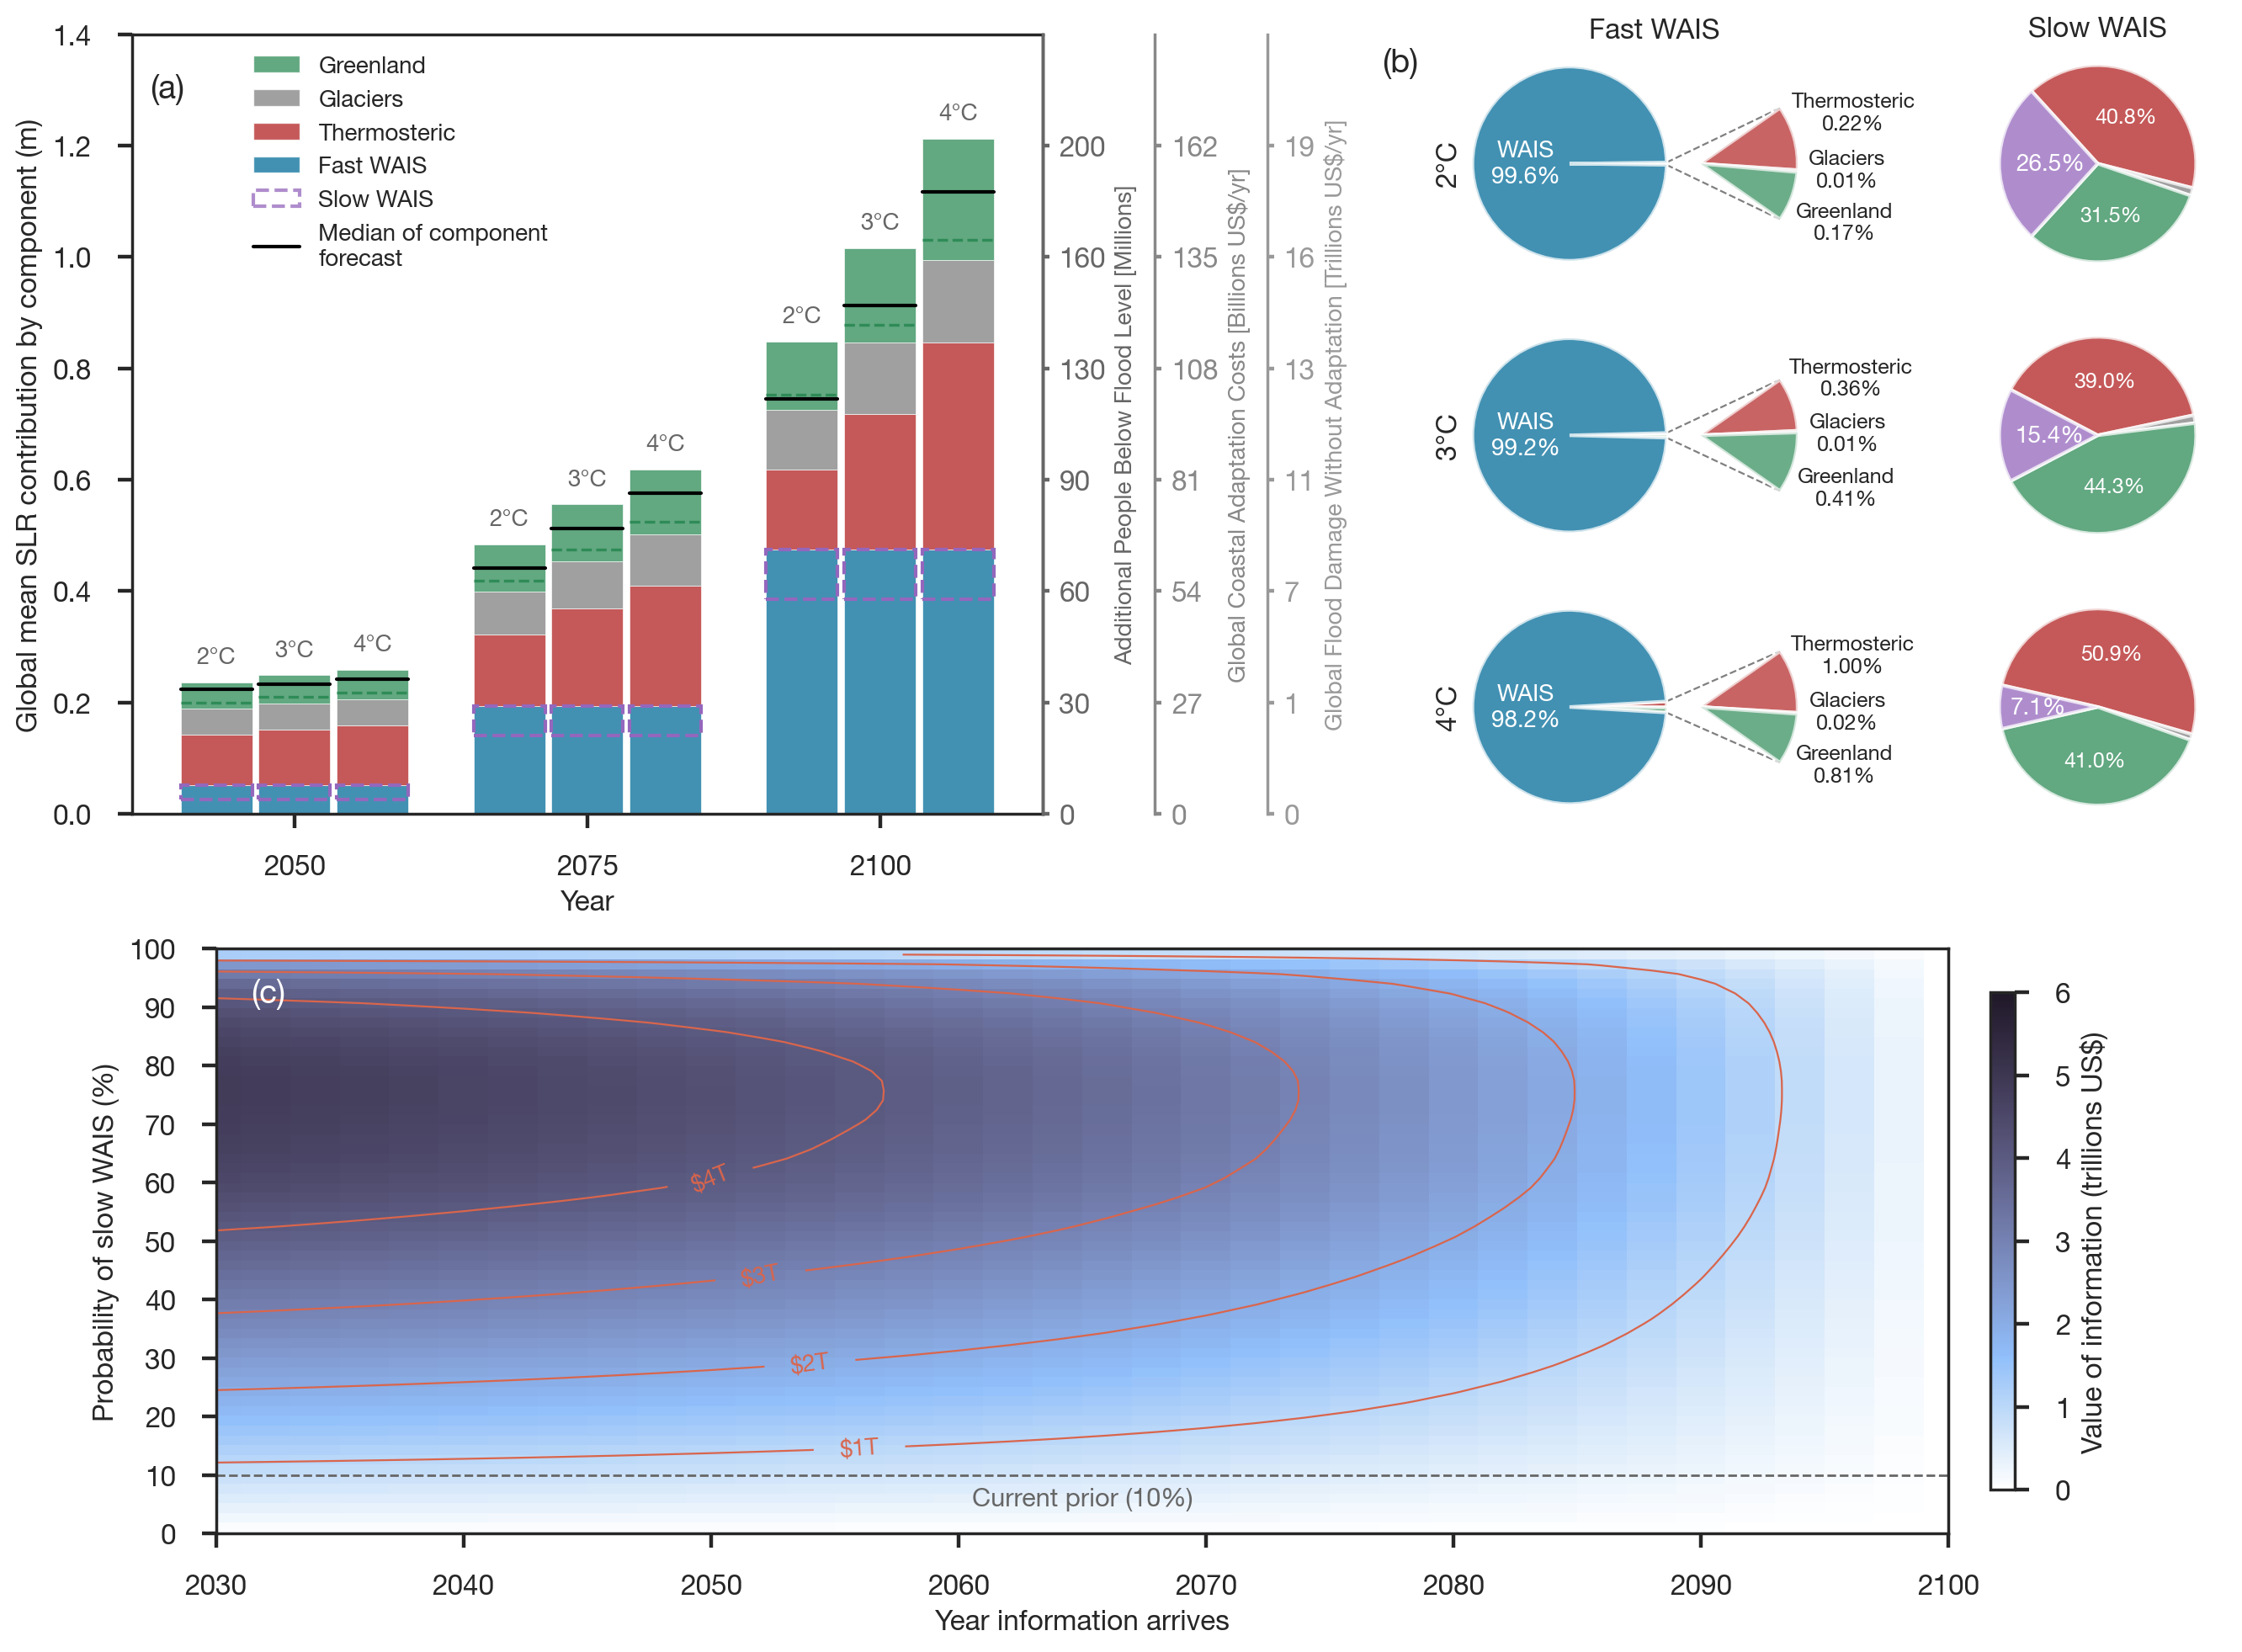
\includegraphics[width=0.66\textwidth]{fig_slr_by_component_v2.png}
%\caption{Where the rise and the uncertainty come from. (a) Average rise from each contributor at three dates and three warming levels. Dashed purple boxes show slow West Antarctic loss. (b) Share of the uncertainty in 2100 from each contributor. West Antarctica dominates if fast loss is possible. (c) The value, in trillions of US dollars, of learning whether West Antarctic loss will be slow or fast. The value is highest when the answer arrives early.}
%\label{fig:leverage}
%\end{figure}

\section{Where the leverage lies}

Knowing the probability of rapid West Antarctic ice loss is the single largest lever for managing sea-level risk. Resolving that question is worth about US\$5 trillion in avoided adaptation costs. The value is largest when confidence in a slow future reaches 75\% and when the answer arrives in time to shape infrastructure decisions. Every year of delay lowers that value. The answer will come from tracking the rate of West Antarctic ice loss over the next two decades. If loss stays near current rates through the 2030s and 2040s, the forecast will narrow toward the lower, emissions-driven range. If loss accelerates, 1.5 to 2 m of rise becomes a planning baseline. These observations require observing systems and research programs sustained at a scale that matches the costs at stake. Even a partial answer would justify research spending far above current levels. Whether intervention could slow this loss is an open question of feasibility, side effects, and governance.

\end{document}
